\chapter{Search for Resonant Di-Higgs }
\label{ch:diHiggs_search}
\section{Introduction and Motivation}
The study of Higgs boson pair production provides a unique opportunity to probe the Higgs self-coupling and to search for physics
beyond the Standard Model (BSM). In the SM, Higgs boson pairs are dominantly produced via gluon-gluon fusion (ggF) through triangle
and box diagrams, as shown in Fig.~\ref{SMLO_ggHH_production}, that exhibit destructive interference.
The predicted cross section for non-resonant di-Higgs production is small, \(0.01449 \pm 0.000019\)~pb,
making this process challenging to observe.
\begin{figure}[!htbp]
    \begin{center}
        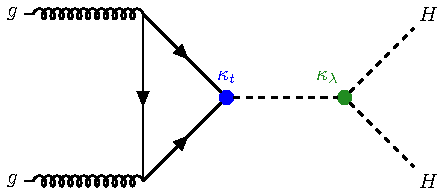
\includegraphics[width=0.45\textwidth]{figures/diHiggsSearches/fey_HH_Triangle.pdf} %
        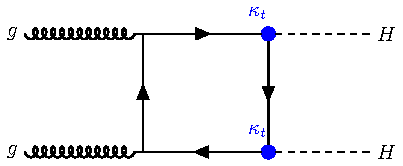
\includegraphics[width=0.45\textwidth]{figures/diHiggsSearches/fey_HH_Box.pdf}
    \end{center}
    \caption{Feynman diagrams for leading-order Higgs boson pair production via gluon fusion}
    \label{SMLO_ggHH_production}
\end{figure}
\begin{figure}[!htbp]
    \begin{center}
        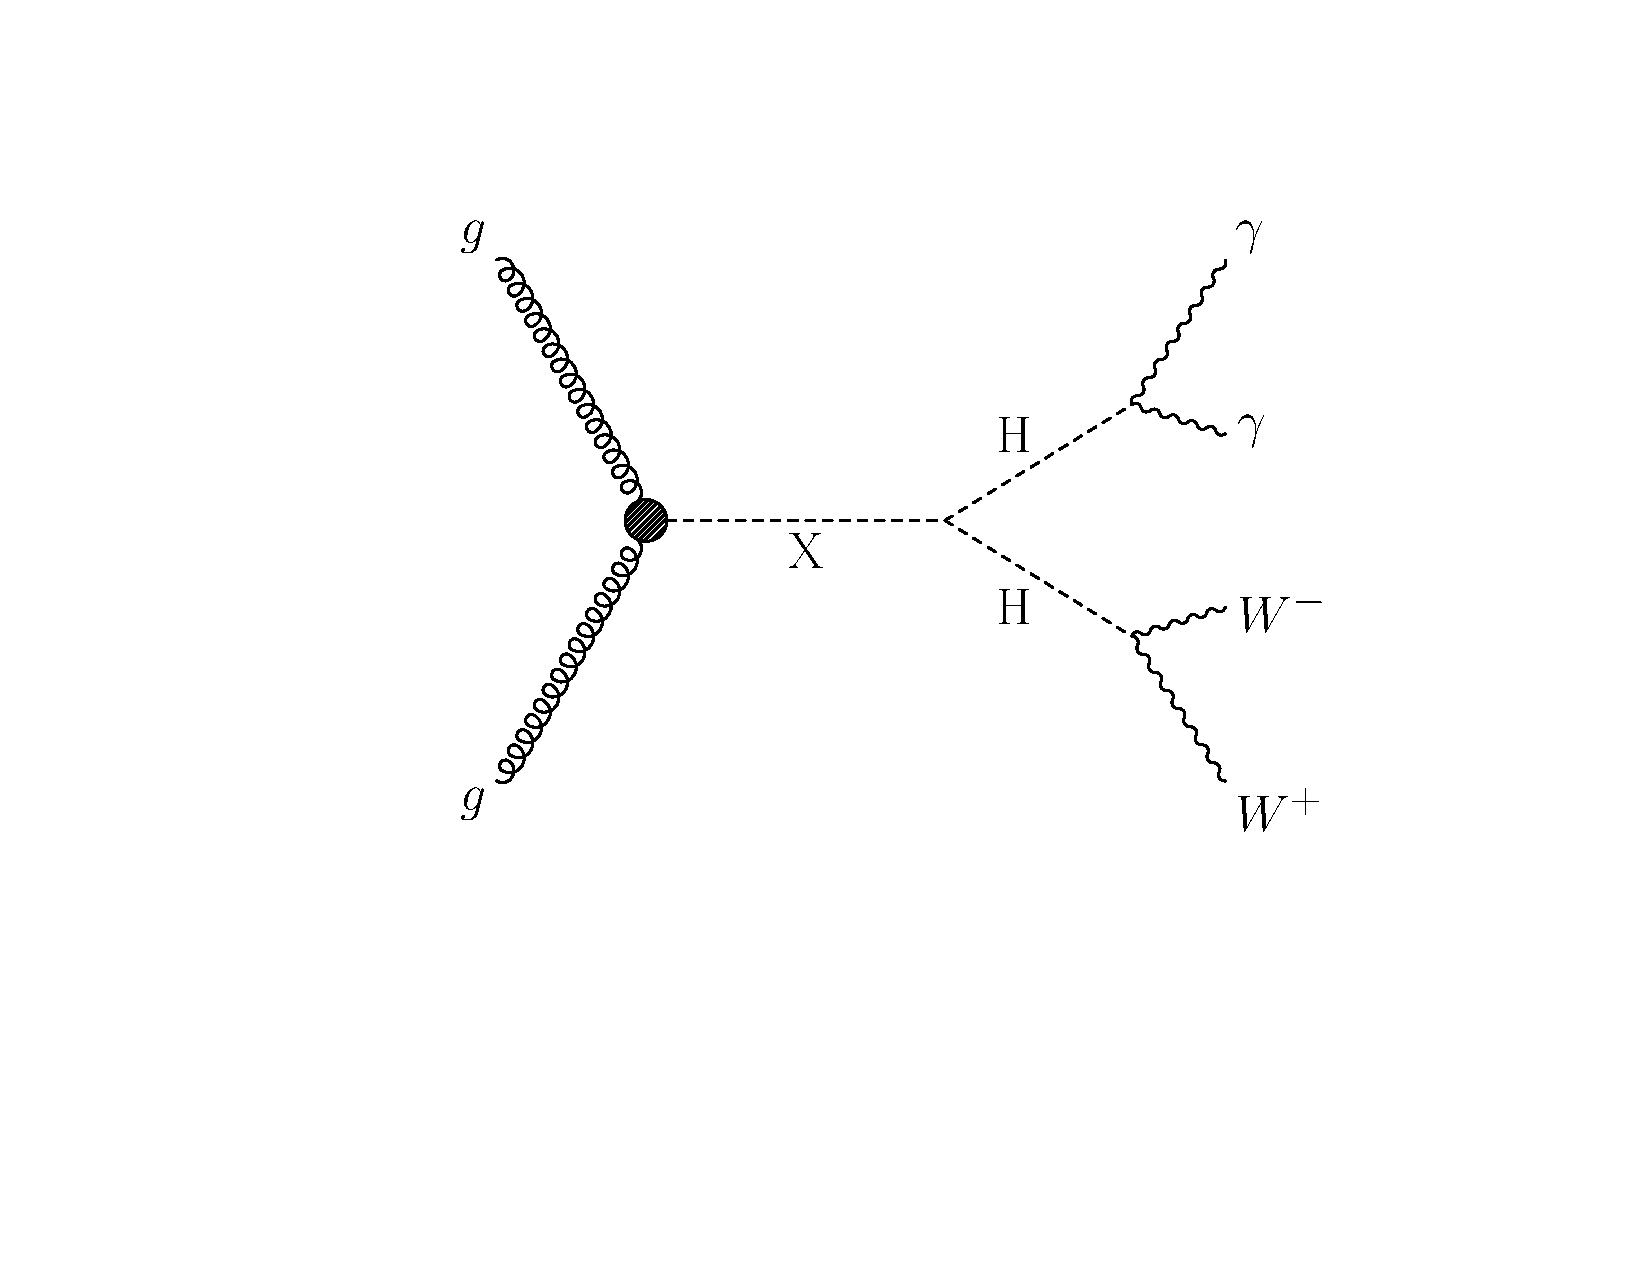
\includegraphics[width=0.45\textwidth]{figures/diHiggsSearches/fey_XHH_HHWWgg.pdf}
    \end{center}
    \caption{Feynman diagram for resonant di-Higgs production in the \HH channel}
    \label{XHHFeynmanDiagram}
\end{figure}


Extensions of the SM, such as the Next-to-Minimal Supersymmetric Standard Model (NMSSM), Randall-Sundrum models, or the two-Higgs
doublet model (2HDM), predict resonant di-Higgs production. In these scenarios, a heavy resonance \(X\) decays into two Higgs
bosons, which subsequently decay into \(WW\) and \(\gamma\gamma\), as shown in Fig.~\ref{XHHFeynmanDiagram}.

This analysis specifically targets the \HHWW channel, utilizing the clean diphoton final state to maximize sensitivity while accounting for all possible jet topologies.
Although this channel has a relatively low branching fraction, as shown in Fig.~\ref{fig:HH_BF},
it provides a distinctive signature for Beyond Standard Model (BSM) searches due to
the presence of a clean diphoton final state combined with couplings to vector bosons.

\begin{figure}[!htbp]
    \centering
    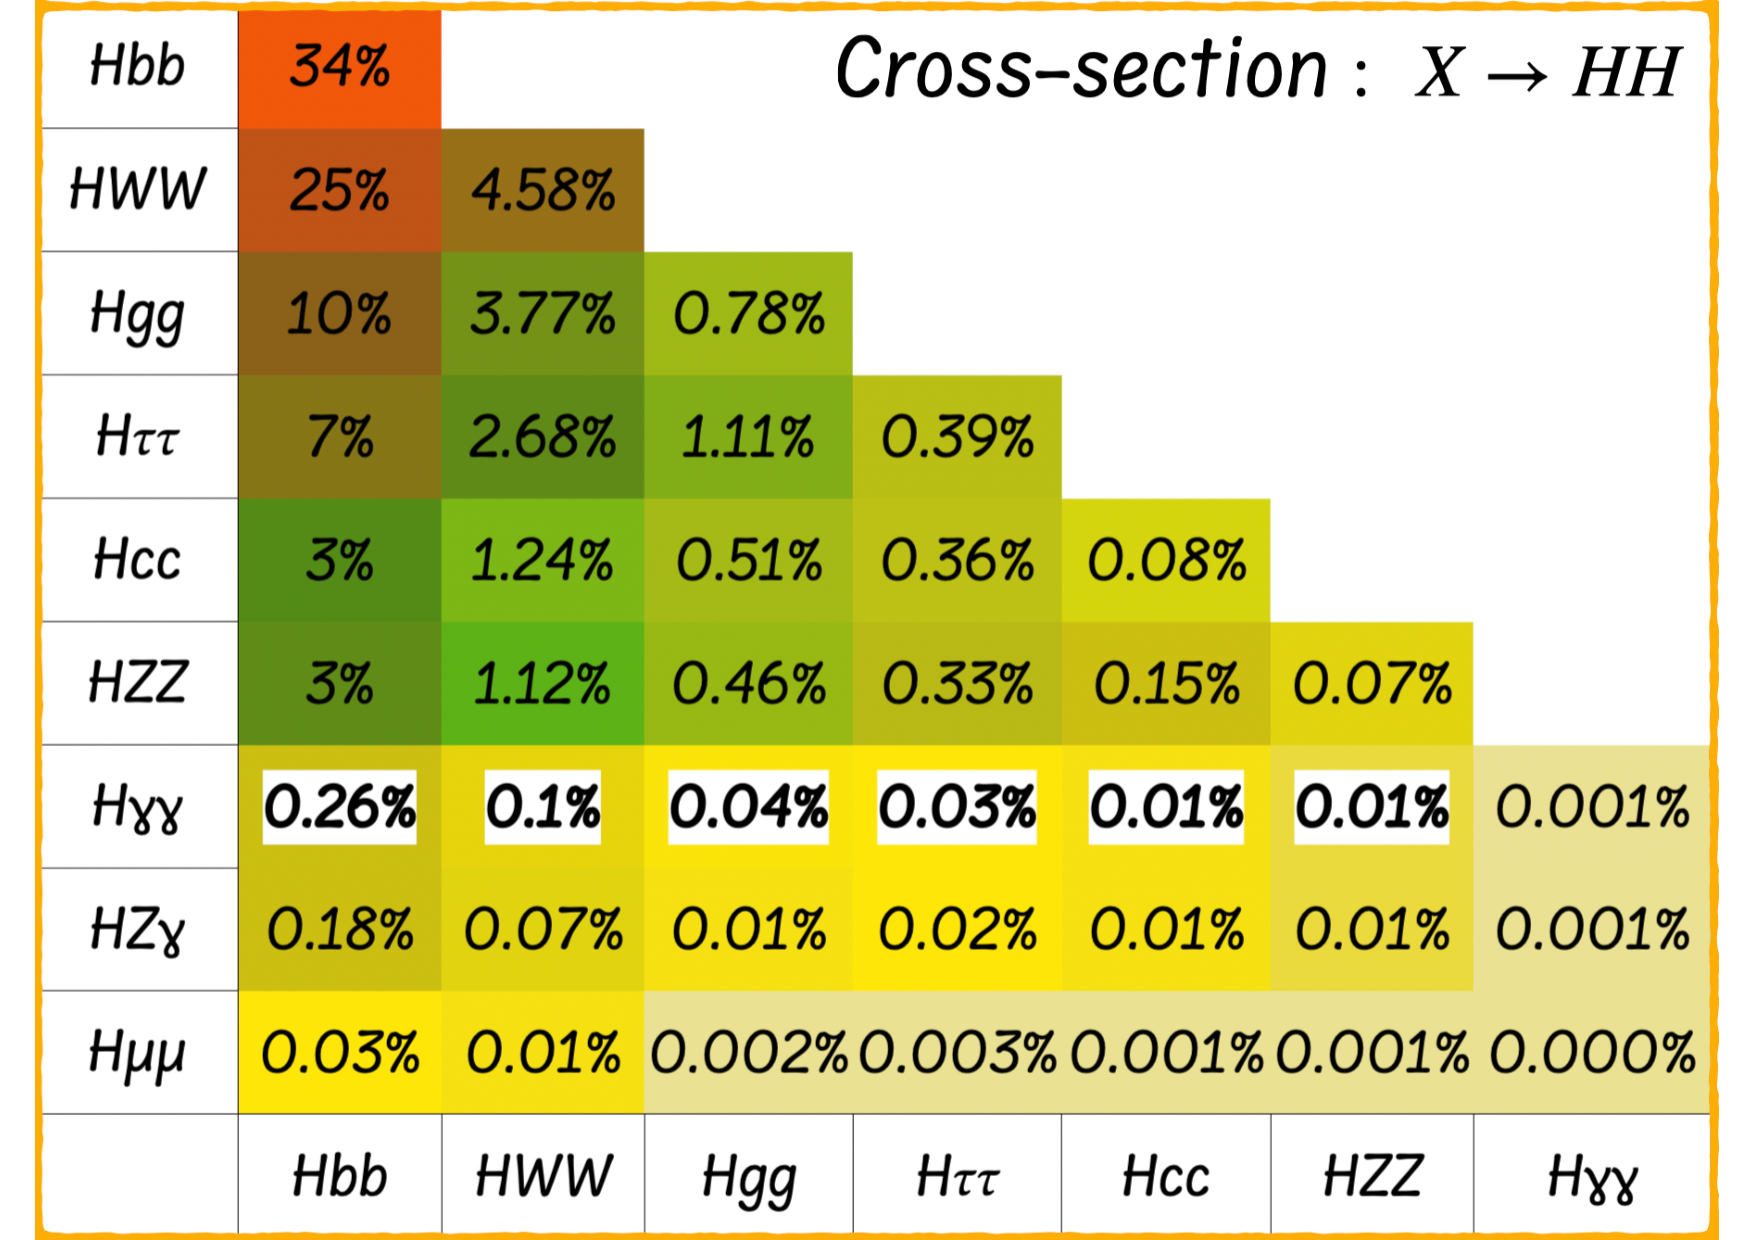
\includegraphics[width=0.95\textwidth]{figures/diHiggsSearches/HH_BF.pdf}
    \caption{Branching fractions of Higgs boson decays.}
    \label{fig:HH_BF}
\end{figure}


\section{Analysis Overview}
The analysis is performed using the full Run-2 Ultra-Legacy dataset, corresponding to an integrated luminosity of 138~fb\(^{-1}\) at
\(\sqrt{s} = 13\)~TeV. The following decay channels are explored:
\begin{itemize}
    \item \textbf{Semi-leptonic (\(l\nu qq\gamma\gamma\)):} One \(W\) boson decays leptonically (\(W \to l\nu\)), and the other
    decays hadronically (\(W \to qq\)).
    \item \textbf{Fully hadronic (\(4q\gamma\gamma\)):} Both \(W\) bosons decay hadronically (\(W \to qq\)).
\end{itemize}

\section{Unique Features of the Analysis}
This analysis includes several innovative aspects:
\begin{itemize}
    \item \textbf{Comprehensive Topology Coverage:} For the first time, all jet topologies are tagged in a single analysis,
    including boosted, semi-boosted, resolved, and cases with leptons reconstructed inside jets.
    \item \textbf{Signal Definition:} We defined our signal as sum of three di-Higgs decay possibilities, i.e.,
    \(HH \to WW\gamma\gamma + ZZ\gamma\gamma + bb\gamma\gamma\).  As the hadronic decay has similar topologies for
    all these three samples and it is challenging to reduce the contamination coming from the other channels ( \(ZZ\gamma\gamma\)
    and \( bb\gamma\gamma\)) into our main signal of interest, which is \(WW\gamma\gamma\).
    Another few important things to note about
    the signal definitions are as follows:
    \begin{itemize}
        \item Analysis is optimized for \HH
        \item For \HH, two decay possibilities for \Wboson are considered, i.e., fully hadronic and semi-leptonic.
        Optimisation of analysis is performed based on these two final states.
        \item For \Zboson\Zboson, as the branching fraction is low for this channel and semi-leptonic contribution is further low. So, the semi-leptonic decay is excluded from the analysis.
        \item The \(bb\gamma\gamma\) channel is added after applying the b-jet veto. This serves two purpose. They are:
        \begin{enumerate}
            \item Reduce the contribution coming from \(bb\gamma\gamma\) channel, hence the limit is driven by the \(WW\gamma\gamma\) not the \(bb\gamma\gamma\) channel.
            \item Our channel become orthogonal to the \(HH \rightarrow bb\gamma\gamma\) analysis.
            \item Furthermore, we are exploiting those events that are rejected by the \(HH \rightarrow bb\gamma\gamma\) analysis. Thus exploiting more information from the same data.
            \item Applying the b-jet veto, also rejects some events from the \(HH\rightarrow ZZ\gamma\gamma\), when \Zboson decays to b-quarks.
        \end{enumerate}
    \end{itemize}
    \item \textbf{Mass Ranges:} The resonance \(X\) is studied in the mass range 250~GeV to 3000~GeV.
    \item \textbf{Leptons Inside Jets:} Events where leptons are reconstructed within jets are included, enhancing sensitivity to
    specific BSM scenarios.
\end{itemize}

\section{Event Selection}
The event selection optimizes sensitivity to semi-leptonic and fully hadronic channels, with the following criteria:

\subsection*{Photon Selection}
\begin{itemize}
    \item A boosted decision tree (BDT) classifier is trained to separate photons from jets~\cite{Sirunyan:2018ouh}.
            The output of this BDT is referred to as the photon ID score
            \footnote{For the boosted regime, where the two photons are close by, the photon ID score was modified to
            account for reduced selection efficiency.
            This modified score is referred to as the ``modified photon ID," detailed in
            Appendix~\ref{appendix:ModifiedPhotonID}}. The photon $ID > -0.7$ is used as a preselection criterion.
    \item Leading photon \(p_T > 35\)~GeV and subleading photon \(p_T > 25\)~GeV.
    \item Photon transverse momentum fractions: \(p_T/m_{\gamma\gamma} > 0.33\) (leading) and \(> 0.25\) (subleading).
    \item Diphoton invariant mass requirement: \(100 < m_{\gamma\gamma} < 180\)~GeV.
\end{itemize}


\subsection*{Lepton Selection}
\begin{itemize}
    \item \textbf{Kinematics:} \(p_T > 10\)~GeV, \(|\eta| < 2.4\), and \(\Delta R(l, \gamma) > 0.4\).
    \item \textbf{\(Z\)-veto:} \(|m_{l\gamma} - 91.2| > 5\)~GeV to suppress contamination from \(Z\)-boson events.
    \item \textbf{ID requirements:}
        \begin{itemize}
            \item \textbf{For isolated electrons:} Use the isolated MVA ID with a signal efficiency of 80\%.
            \item \textbf{For isolated muons:} Require global muons with tight ID and an isolation threshold of 0.15.
            \item \textbf{For non-isolated electrons:} Use the non-isolated MVA ID with a signal efficiency of 80\%, ensuring \(\Delta R < 0.8\) with a good FatJet (as defined in the jet selection).
            \item \textbf{For non-isolated muons:} Require high \(p_T\) ID\todo[fancyline]{define High pT ID} without isolation criteria, ensuring \(\Delta R < 0.8\) with a good FatJet (as defined in the jet selection\todo[fancyline]{cite jet section}).
        \end{itemize}
\end{itemize}

\subsection*{Small Radius Jets (AK4 CHS)}
\begin{itemize}
    \item \textbf{ID:} Tight
    \item \textbf{PU Jet ID:} Tight
    \item \textbf{Kinematics:} \(p_T > 20\)~GeV, \(|\eta| < 2.4\)
    \item \textbf{Separation criteria:}
        \begin{itemize}
            \item \(\Delta R(\gamma, \text{jet}) > 0.4\)
            \item \(\Delta R(\text{Isolated Lepton, jet}) > 0.4\)
        \end{itemize}
\end{itemize}

\subsection*{FatJets (AK8 PUPPI)}
\begin{itemize}
    \item \textbf{Kinematics:} \(p_T > 100~\text{GeV}, |\eta| < 2.4\), with Tight Jet ID.
    \item \textbf{Separation criteria:}
    \begin{itemize}
        \item \(\Delta R(\gamma, \text{jet}) > 0.8\).
    \end{itemize}
    \item \textbf{Boosted \(H_{bb}\) jet veto:} \(X_{bb}/X_{\text{qcd}} < 0.9\).
    \item \textbf{Fully Hadronic Higgs Jet:}
    \begin{itemize}
        \item Particle Transformer\todo{define particle transformer in the footnote} Higgs Tagging score \(> 0.2\).
    \end{itemize}
    \item \textbf{Semi-Leptonic Higgs Jet:}
    \begin{itemize}
        \item \(\Delta R(\text{Non-isolated lepton}, \text{FatJet}) < 0.8\).
    \end{itemize}
    \item \textbf{Boosted \(W\)-Jet:}
    \begin{itemize}
        \item ParticleNet\todo{define particleNet in the footnote} loose working point for W-jet tagging.
        \item \(\Delta R(\text{Isolated leptons}, \text{FatJet}) > 0.8\).
    \end{itemize}
\end{itemize}

\subsection*{Event Selection}
The event selection is optimized for the semi-leptonic and fully hadronic channels and is summarized in Fig.~\ref{fig:event_selection_workflow}.
\begin{figure}[!htbp]
    \centering
    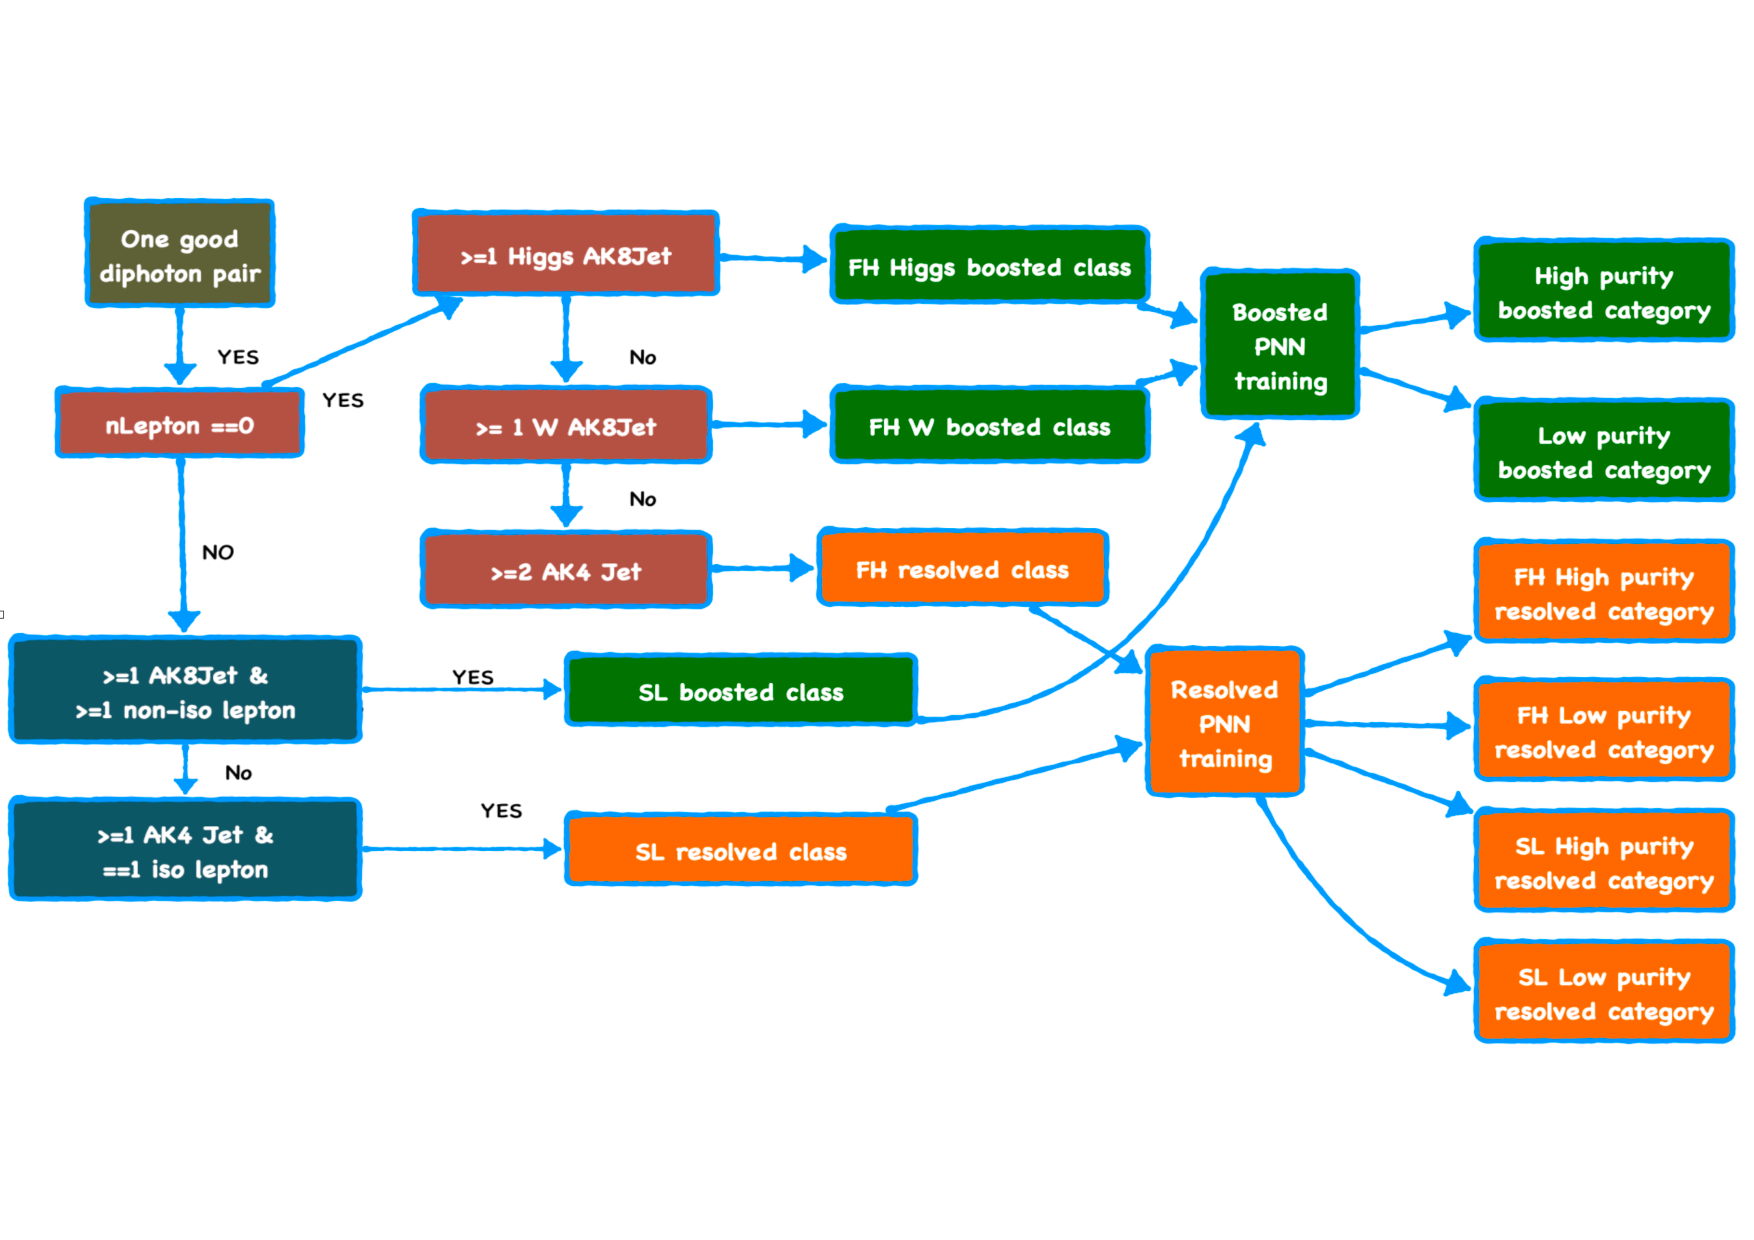
\includegraphics[width=0.95\textwidth]{figures/diHiggsSearches/EventSelectionWorkflow.pdf}
    \caption{Event selection workflow for the \HHWW analysis.}
    \label{fig:event_selection_workflow}
\end{figure}


\section{Data-Driven Background Estimation}
Accurately estimating background processes is crucial for isolating the \HHWW signal.
The dominant backgrounds include non-resonant diphoton production, single Higgs processes, and multijet events
where fake photons mimic the signal.
A data-driven approach is used to estimate fake photon contributions~\cite{CMS:2020cga}.

\subsection{Motivation}
The limited statistics of QCD Monte Carlo (MC) samples lead to poor modeling of key input features for multivariate analyses.
To ensure reliable machine learning training and data-MC agreement, a data-driven method is adopted~\cite{CMS:2020cga}.
This approach uses events from the photon ID MVA sideband to model fake photon contributions.

\subsection{Methodology}
The data-driven background estimation follows these steps:
\begin{enumerate}
    \item \textbf{Photon ID Sideband Selection:}
    Events failing the photon ID MVA preselection cut are used to model fake photons.
    The sideband regions are defined as:
    \begin{itemize}
        \item Resolved category: Photon ID MVA in \([-0.9, -0.7]\).
        \item Boosted category: Photon ID MVA in \([-0.95, -0.9]\).
    \end{itemize}

    \item \textbf{PDF Generation for Fake Photons:}
    A probability density function (PDF) for the photon ID MVA distribution of fake photons is
    derived from MC samples (e.g., \(\gamma + \text{jets}\)).
    Sideband events are reweighted to match the PDF in the signal region.

    \item \textbf{Reweighting and Normalization:}
    Per-event weights are applied to sideband events to reshape the photon ID MVA distribution.
    The weight \(w\) is defined as:
    \[
        w = \frac{\int_{\text{minID}}^{\text{maxID}} \text{fakePDF}(x) \, dx}
                 {\int_{\text{sidebandMinID}}^{\text{sidebandMaxID}} \text{fakePDF}(x) \, dx}.
    \]
    Separate weights are applied for resolved and boosted categories.

    \item \textbf{Validation:}
    The reweighted MC is normalized to data, and comparisons before and after reweighting show improved agreement in key variables like \(m_{\gamma\gamma}\).
\end{enumerate}

\subsection{Challenges and Solutions}
Despite its success, this method presents some challenges:
\begin{itemize}
    \item \textbf{Muon Channel in Semi-Leptonic (SL) Events:}
    While the method improves agreement in the electron channel, it worsens the muon channel.
    Potential solutions include:
    \begin{itemize}
        \item Applying the data-driven approach only to the electron channel.
        \item Using separate reweighting for electron and muon channels.
    \end{itemize}
    For now, we are using the additional MVA reweighting on top of this method to improve the overall agreement. As we don't use the MC for the signal extraction, the impact of this method on the signal extraction is minimal.

    \item \textbf{Photon ID Sidebands:}
    Key assumptions in this method include:
    \begin{enumerate}
        \item Photon ID MVA has minimal correlation with other analysis variables.
        \item The sideband is dominated by fake photons (e.g., QCD and \(\gamma + \text{jets}\)).
        \item Sideband photons are assumed to be entirely fake.
    \end{enumerate}
\end{itemize}

\subsection{Implementation in Different Channels}
The method is applied to both fully hadronic (FH) and semi-leptonic (SL) channels:
\begin{itemize}
    \item \textbf{Fully Hadronic Channel:}
    Dominated by QCD backgrounds, with the photon ID sideband effectively modeling fake photon contributions.
    \item \textbf{Semi-Leptonic Channel:}
    Includes contributions from \(W\gamma\gamma\) and \(t\bar{t}\) processes, with non-isolated leptons playing a key role in background estimation.
\end{itemize}

\subsection{Impact of the Data-Driven Method}
The data-driven background estimation significantly improves the analysis:
\begin{itemize}
    \item Enhanced modeling of photon-related variables in resolved and boosted categories.
    \item Improved agreement between data and MC in control regions, as shown in Fig.~\ref{fig:control_plots}.
        \begin{figure}[!htbp]
            \centering
            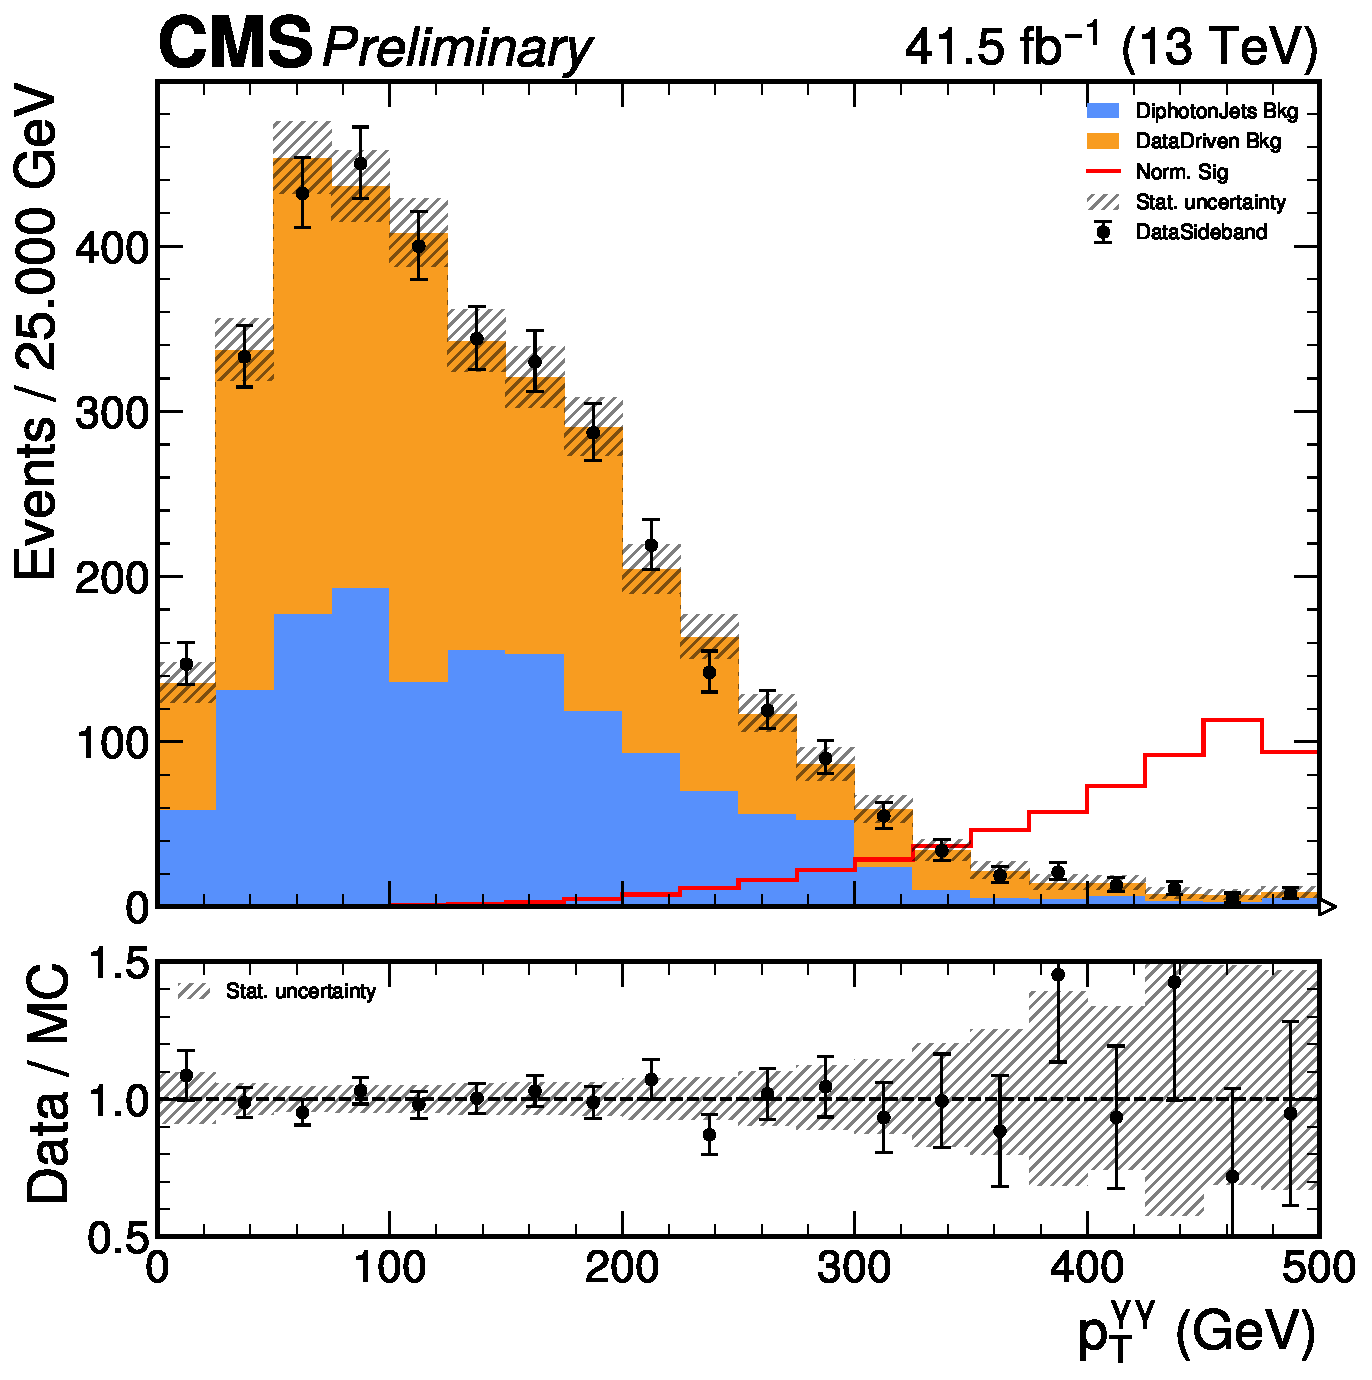
\includegraphics[width=0.45\textwidth]{figures/ControlPlots/boosted_PNN_reweighted/PNN_Diphoton_pt_after_reweight.pdf}%
            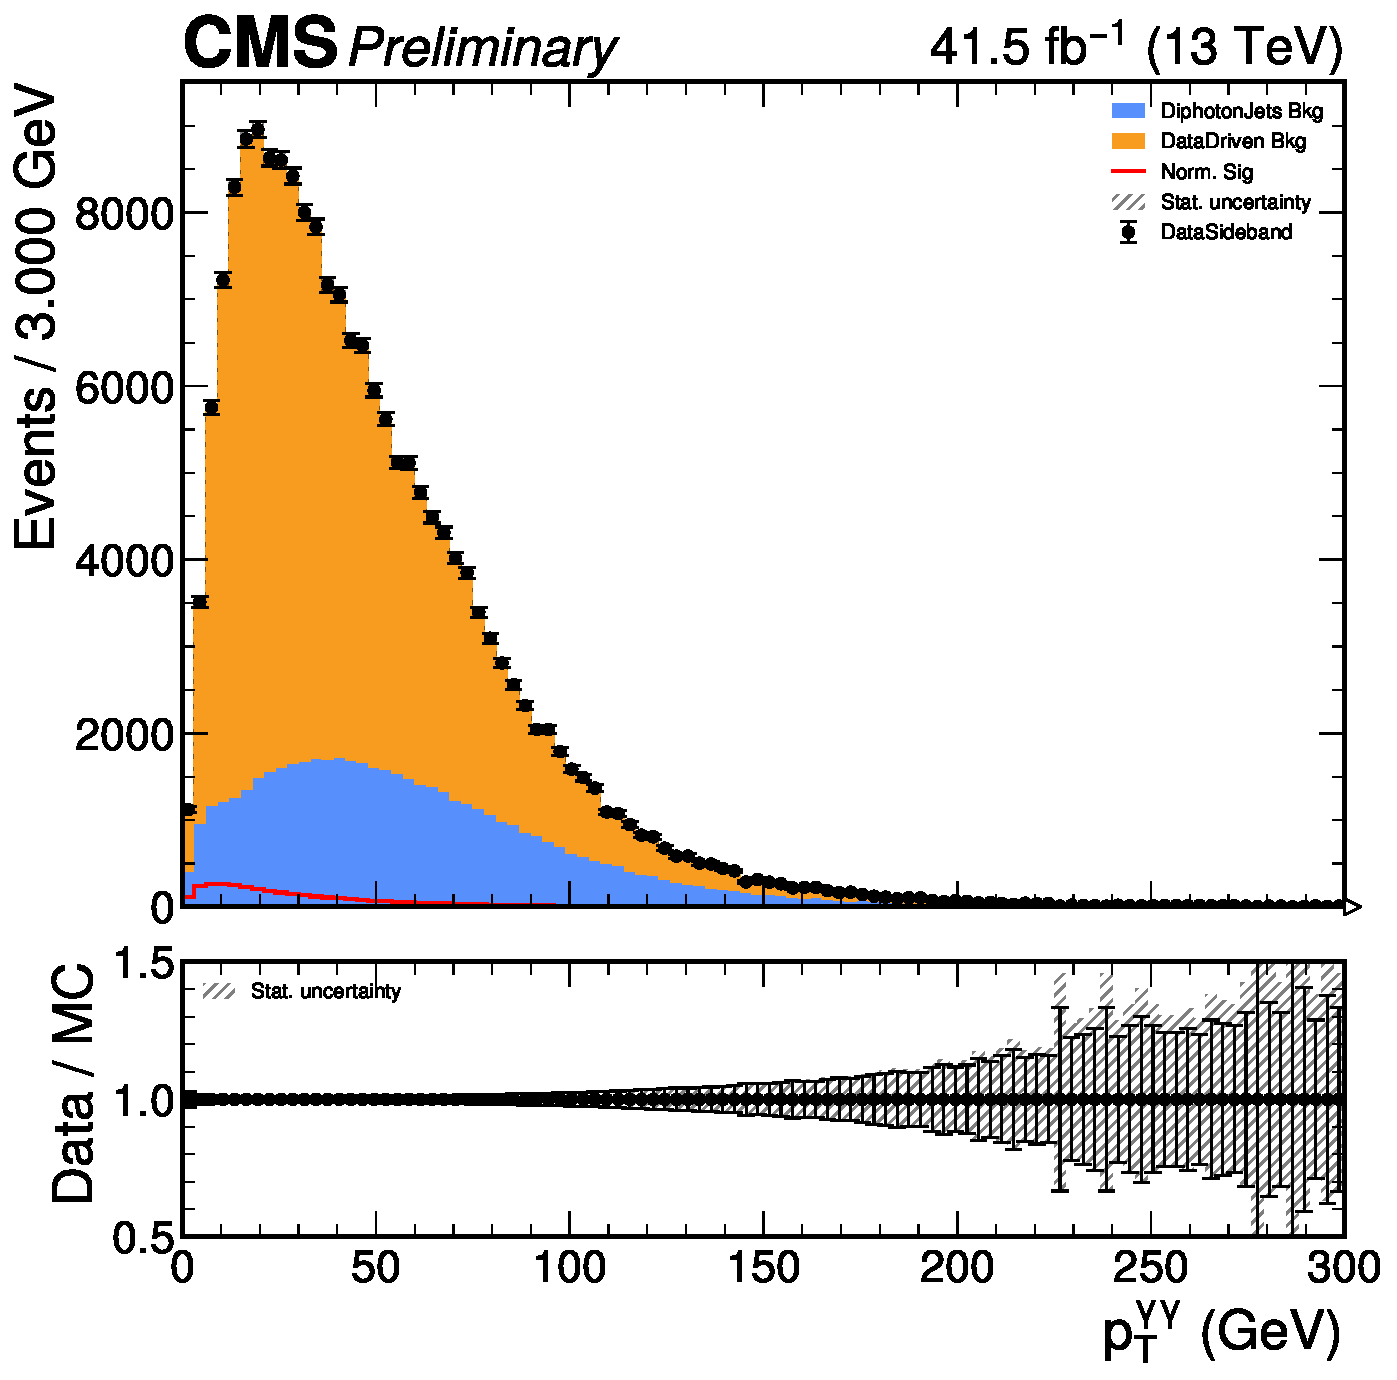
\includegraphics[width=0.45\textwidth]{figures/ControlPlots/resolved_PNN_reweighted/PNN_Diphoton_pt.pdf}
            \caption{Control plots showing the agreement between data and MC after applying the data-driven method. Left: Boosted category. Right: Resolved category.}
            \label{fig:control_plots}
        \end{figure}
\end{itemize}

\section{Multivariate Analysis Using Parameterized Neural Network (pNN)}
To maximize the sensitivity of the search for resonant \HHWW, a multivariate analysis (MVA) is performed
using a Parameterized Neural Network (pNN). The pNN method allows for simultaneous training across multiple signal hypotheses,
parameterized by the mass of the heavy resonance \(m_X\). This approach ensures a robust discrimination between signal and
background across a wide range of masses, from 250~GeV to 3000~GeV.

The pNN is implemented as a deep feed-forward neural network. Its inputs include kinematic and topological features of the events, with the resonance mass \(m_X\) incorporated as a parameter to generalize across different signal hypotheses. The network is trained using the Adam optimizer with stochastic gradient descent, and GPU acceleration is used for efficient processing of large datasets. Additional features, such as dropout layers, are included to prevent overfitting and enhance model generalization.

Separate pNNs are trained for the boosted and resolved topologies to account for the distinct event kinematics in these categories.
The boosted category includes events where \(W\)-bosons' decay products are merged into single AK8 jets, while the resolved category reconstructs \(W\)-bosons' decay products as individual AK4 jets.
Input features, such as photon, jet, and missing transverse energy (\(E_T^{\text{miss}}\)) observables, are carefully selected based on their ability to discriminate signal from background. These features include variables like the diphoton \(p_T/m_{\gamma\gamma}\), the angular separation (\(dR\)) between photons, and jet kinematics. The full list of input variables used for the boosted pNN training is provided in Table~\ref{tab:inputvariables_boosted} and for the resolved pNN training in Table~\ref{tab:inputvariables_resolved}.
\begin{table}[htbp!]
    \centering
    \begin{tabularx}{\textwidth}{|l|X|}
    \hline
    \textbf{Feature} & \textbf{Description} \\
    \hline
    Diphoton\_pTom & Transverse momentum of the diphoton system over the mass of the diphoton system \\
    Diphoton\_dR & Delta R between the two photons \\
    Diphoton\_eta & Pseudorapidity of the diphoton system \\
    Diphoton\_phi & Azimuthal angle of the diphoton system \\
    LeadPhoton\_pTom & Transverse momentum of the leading photon over the mass of the diphoton system \\
    SubleadPhoton\_pTom & Transverse momentum of the subleading photon over the mass of the diphoton system \\
    LeadPhoton\_eta & Pseudorapidity of the leading photon \\
    LeadPhoton\_phi & Azimuthal angle of the leading photon \\
    SubleadPhoton\_eta & Pseudorapidity of the subleading photon \\
    SubleadPhoton\_phi & Azimuthal angle of the subleading photon \\
    fatjet\_1\_pT & Transverse momentum of the leading fatjet \\
    fatjet\_1\_eta & Pseudorapidity of the leading fatjet \\
    fatjet\_1\_phi & Azimuthal angle of the leading fatjet \\
    fatjet\_1\_mass & Mass of the leading fatjet \\
    fatjet\_2\_pT & Transverse momentum of the subleading fatjet \\
    fatjet\_2\_eta & Pseudorapidity of the subleading fatjet \\
    fatjet\_2\_phi & Azimuthal angle of the subleading fatjet \\
    fatjet\_2\_mass & Mass of the subleading fatjet \\
    fatjet\_1\_2\_dR & Delta R between the two fatjets \\
    fatjet\_1\_diphoton\_dR & Delta R between the leading fatjet and the diphoton system \\
    fatjet\_2\_diphoton\_dR & Delta R between the subleading fatjet and the diphoton system \\
    fatjet\_1\_leadphoton\_dR & Delta R between the leading fatjet and the leading photon \\
    fatjet\_1\_subleadphoton\_dR & Delta R between the leading fatjet and the subleading photon \\
    fatjet\_2\_leadphoton\_dR & Delta R between the subleading fatjet and the leading photon \\
    fatjet\_2\_subleadphoton\_dR & Delta R between the subleading fatjet and the subleading photon \\
    max\_fatjets\_mass & Maximum mass of the two fatjets \\
    nGoodAK4jets & Number of good AK4 jets \\
    nGoodAK8jets & Number of good AK8 jets \\
    Third leading jets\_pT & Transverse momentum of the third leading jets \\
    Third leading jets\_eta & Pseudorapidity of the third leading jets \\
    Third leading jets\_phi & Azimuthal angle of the third leading jets \\
    Third leading jets\_mass & Mass of the third leading jets \\
    PuppiMET\_pt & Transverse momentum of the missing transverse energy \\
    dphi\_jet1\_PuppiMET & Azimuthal angle difference between the first jet and missing transverse energy \\
    dphi\_jet2\_PuppiMET & Azimuthal angle difference between the second jet and missing transverse energy \\
    PuppiMET\_sumEt & Sum of the transverse energy of the missing transverse energy \\
    MX & Invariant mass of the resonance X \\
    \hline
    \end{tabularx}
    \caption{Input variables used for the boosted PNN training.}
    \label{tab:inputvariables_boosted}
\end{table}
\begin{table}[htbp!]
    \centering
    \begin{tabularx}{\textwidth}{|l|X|}
    \hline
    \textbf{Feature} & \textbf{Description} \\
    \hline
    MX & Invariant mass of the resonance X \\
    Diphoton\_pTom & Transverse momentum of the diphoton system over the mass of the diphoton system \\
    Diphoton\_eta & Pseudorapidity of the diphoton system \\
    Diphoton\_phi & Azimuthal angle of the diphoton system \\
    LeadPhoton\_pTom & Transverse momentum of the leading photon over the mass of the diphoton system \\
    SubleadPhoton\_pTom & Transverse momentum of the subleading photon over the mass of the diphoton system \\
    LeadPhoton\_eta & Pseudorapidity of the leading photon \\
    LeadPhoton\_phi & Azimuthal angle of the leading photon \\
    SubleadPhoton\_eta & Pseudorapidity of the subleading photon \\
    SubleadPhoton\_phi & Azimuthal angle of the subleading photon \\
    Diphoton\_dR & Delta R between the two photons \\
    Diphoton\_dEta & Delta pseudorapidity between the two photons \\
    jet\_1\_2\_pt & Transverse momentum of the combined leading and subleading jets \\
    jet\_1\_2\_mass & Mass of the combined leading and subleading jets \\
    jet\_1\_2\_dR & Delta R between the leading and subleading jets \\
    jet\_1\_pt & Transverse momentum of the leading jet \\
    jet\_2\_pt & Transverse momentum of the subleading jet \\
    photon1\_jet1\_dR & Delta R between the leading photon and the leading jet \\
    photon1\_jet2\_dR & Delta R between the leading photon and the subleading jet \\
    photon1\_jet1\_2\_dR & Delta R between the leading photon and the combined leading and subleading jets \\
    Diphoton\_jet1\_2\_dR & Delta R between the diphoton system and the combined leading and subleading jets \\
    Diphoton\_jet1\_dR & Delta R between the diphoton system and the leading jet \\
    Diphoton\_jet2\_dR & Delta R between the diphoton system and the subleading jet \\
    photon2\_jet1\_dR & Delta R between the subleading photon and the leading jet \\
    photon2\_jet2\_dR & Delta R between the subleading photon and the subleading jet \\
    photon2\_jet1\_2\_dR & Delta R between the subleading photon and the combined leading and subleading jets \\
    Diphoton\_jet\_1\_2\_dEta & Delta pseudorapidity between the diphoton system and the combined leading and subleading jets \\
    Diphoton\_jet\_1\_dEta & Delta pseudorapidity between the diphoton system and the leading jet \\
    Diphoton\_jet\_2\_dEta & Delta pseudorapidity between the diphoton system and the subleading jet \\
    Diphoton\_jet\_1\_2\_dPhi & Delta phi between the diphoton system and the combined leading and subleading jets \\
    Diphoton\_jet\_1\_dPhi & Delta phi between the diphoton system and the leading jet \\
    Diphoton\_jet\_2\_dPhi & Delta phi between the diphoton system and the subleading jet \\
    PuppiMET\_pt & Transverse momentum of the missing transverse energy \\
    nGoodAK4jets & Number of good AK4 jets \\
    nGoodisoleptons & Number of good isolated leptons \\
    leading\_bscore & B-tagging score of the leading jet \\
    subleading\_bscore & B-tagging score of the subleading jet \\
    sum\_two\_max\_bscores & Sum of the two highest b-tagging scores \\

    \hline
    \end{tabularx}
    \caption{Input variables used for the resolved PNN training.}
    \label{tab:inputvariables_resolved}
\end{table}

The performance of the pNN is evaluated using metrics such as the area under the curve (AUC) and signal-to-background ratio improvements. The pNN demonstrates significant enhancement in discrimination between signal and background across the entire mass range. Feature importance plots highlight the critical role of variables such as diphoton \(p_T/m_{\gamma\gamma}\) and photon angular separations in improving sensitivity. Separate training for the boosted and resolved categories further optimizes the analysis for these topologies.

The output of the pNN serves as the final discriminant for signal extraction in the \(m_{\gamma\gamma}\) distribution. By combining the boosted and resolved categories, the analysis achieves a 60\% improvement in sensitivity compared to previous results. Control plots of key variables before and after applying the pNN show excellent agreement between data and Monte Carlo, validating the robustness of the method.

The parameterized neural network approach thus provides a powerful framework for signal extraction in the \HHWW analysis. By training across multiple mass hypotheses and incorporating advanced multivariate techniques, the pNN significantly improves the sensitivity to resonant di-Higgs production, particularly in high-mass regions.

\section{Signal and background modelling}
\label{sec:AnalyticFitting}

For the statistical interpretation of the data, a parametric fit to the \mgg distribution of the event signal candidates is performed.
The template \mgg distributions of the HH and single-H processes are modeled using the simulated MC events, while the continuum background is modeled from data.

\subsection{HH and single-Higgs modeling}
\label{sec:SignalFitting}
Signal shapes for the invariant mass distribution of the diphoton candidate are derived for each process separately by category and data-taking year.

Signal models are formed by an analytic fit of a sum of up to five Gaussians to a binned $\mgg$ distribution.
The fit for the top two highest DNN score region are shown in Fig.~\ref{fig:smodel_combineFHSL_cat12highpurity_MX3000}.
\begin{figure}[!htbp]
    \centering
    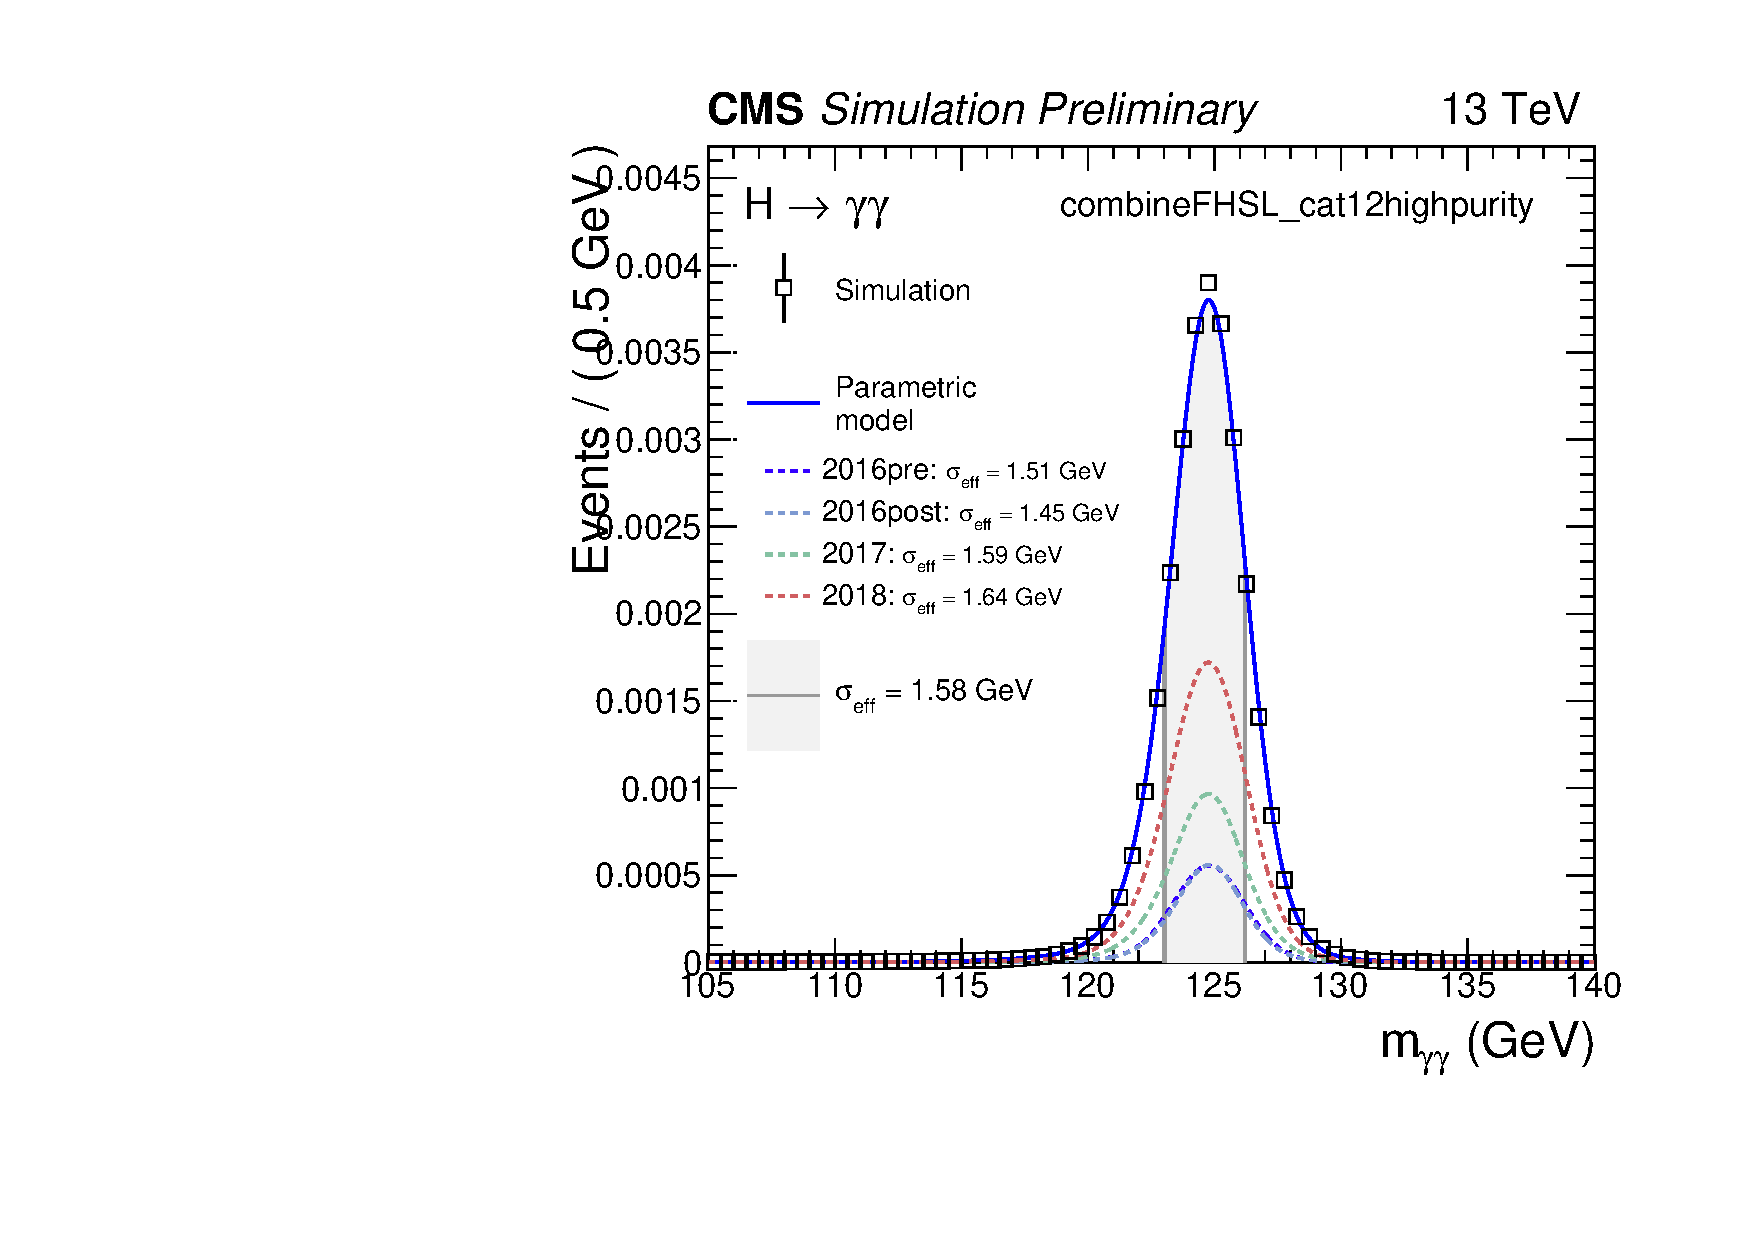
\includegraphics[width=0.45\textwidth]{figures/Signal_Modeling/MX3000_MH125_smodel_combineFHSL_cat12highpurity.pdf}%
    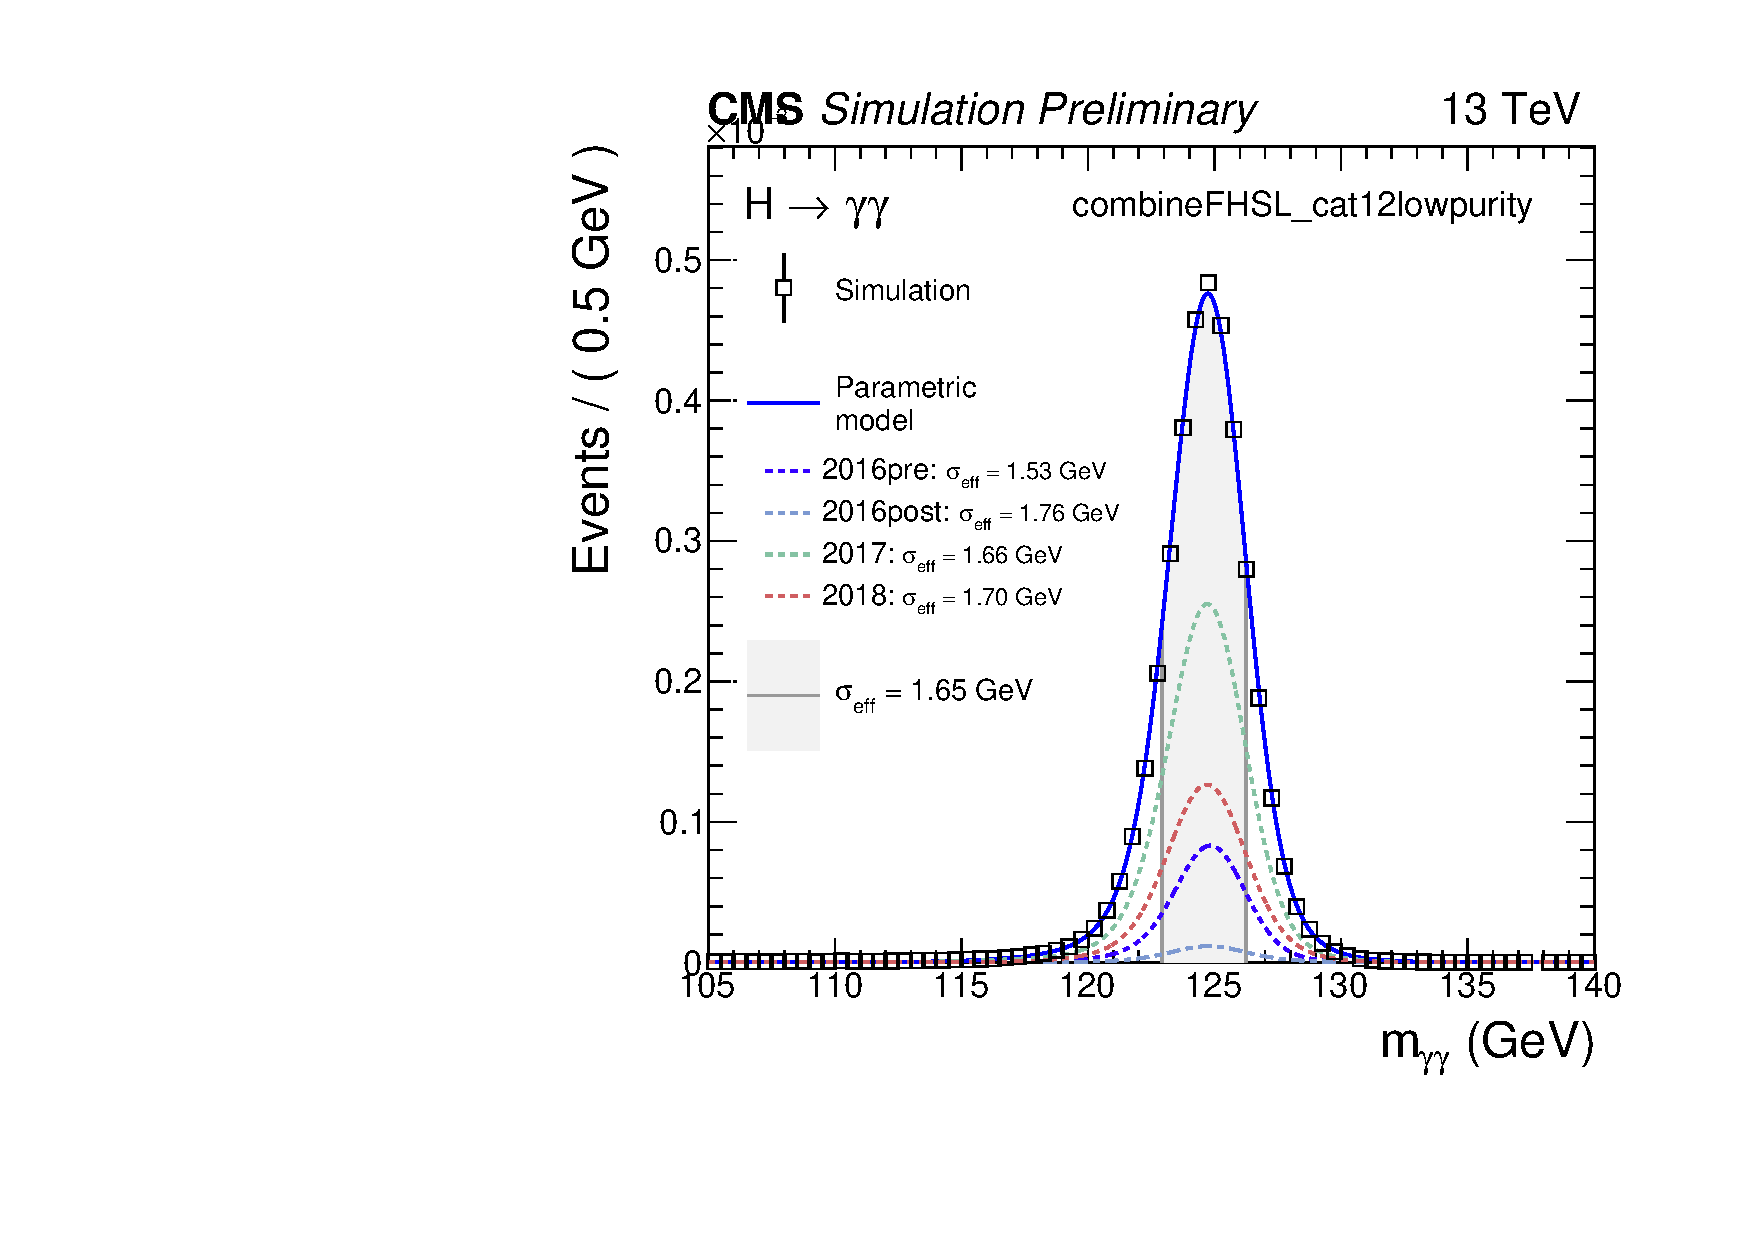
\includegraphics[width=0.45\textwidth]{figures/Signal_Modeling/MX3000_MH125_smodel_combineFHSL_cat12lowpurity.pdf}
    \caption{PNN high (Left) and low purity (Right) categories for $M_X = 3000$ GeV.}
    \label{fig:smodel_combineFHSL_cat12highpurity_MX3000}
\end{figure}


The effects of anomalous $\kappa_{\lambda}$ values on the Higgs boson branching ratios and on the single Higgs cross sections
are taken into account using the modeling provided in Reference \cite{Degrassi:2016wml} and \cite{Maltoni:2017ims}.

% \subsection{Single Higgs background}

% There are expected resonant background processes present in the signal region, $115 < \mgg < 135$ GeV, due to $H\rightarrow\gamma\gamma$ processes, which cannot be modeled with a data-driven
% method using data sideband events. These backgrounds are modeled with MC in the same fashion as the $HH\rightarrow WW\gamma\gamma$ signals as described in Section \ref{sec:SignalFitting}. The single higgs
% processes considered as resonant backgrounds are the gluon-gluon fusion, vector boson fusion, associated production with a vector boson, and associated production with a top quark pair (ttH), where the Higgs boson decays
% into two photons. A separate fit is made for each analysis category and production mode. For cases in which there is a very small number of MC statistics, the diphoton shape from
% the di-Higgs signal model in the same analysis category is taken and scaled to the single higgs yield in this category, and used to model the single higgs shape in this category.

\subsection{Continuum background}
\label{sec:AnalyticFitting_Background}

The continuum background in the \mgg distribution is modelled from data using the discrete profiling method \cite{Dauncey_2015} to account for the uncertainty related to the background shape.
This method treats the choice of the background parametrization as a discrete nuisance parameter. The parametric function is selected among a set of function families providing a complete
description of smoothly falling backgrounds.

% A data-driven background model is produced for each category using the data sidebands in the regions $100 < \mgg < 115$ GeV and $135 < \mgg < 180$ GeV.
% The aim of this is to model the continuum background.
% After the event selections and categorizations described in Section \ref{sec:event_selection} are applied, analytic functions are fit to the resulting $\mgg$ distributions in the data sidebands for each category.
% These are later combined with their corresponding signal models in order to extract final results.
% As with the signal fitting, an F-Test is performed first in order to obtain initial best-fit estimates for backgrounds functions to the data-sidebands, and to determine which functions will be considered.
% Bernstein, laurent, exponential, and powerlaw function families are considered as
% candidates to fit the data, and F-Tests are performed for each of these. The three data taking years are merged together before the F-test and function fitting is performed.
% After determining which functions pass the F-Test, a best fit function is chosen with the envelope method by treating the choice of function as a discrete nuisance parameter.
% An uncertainty is then assigned to the chosen fit function based on a combination of the likelihoods of all attempted fit functions. This method is described in
% Reference \cite{Dauncey_2015}.

% After obtaining signal models, continuum background models and Single-Higgs models for each final state, a signal plus background fit is performed.
% The combination of all categories' signal plus background fits in the range 100 $<$ $\mgg$ $<$ 180 GeV, where each category is weighted by S$/$(S$+$B), is shown in Figure \ref{fig:Run2SplusB}.

% \begin{figure}[!htbp]
%   \centering
%   \includegraphics[width=0.55\textwidth]{Images/Results/All_combined_SplusB.pdf}
%  \caption{The observed diphoton mass distribution including the signal plus background fit (red), the Single-Higgs + continuum background fit (blue) and the continuum background (black dashed line),
%  with bands covering the $\pm 1\sigma$ and $\pm 2\sigma$ uncertainties in the fitted background. All analysis categories are combined and weighted by S$/$(S$+$B).}
%   \label{fig:Run2SplusB}
% \end{figure}

\section{Results}
\label{sec:results}

This analysis conducted presents the first search for the resonant production
of Higgs boson pairs (HH) in
the $WW\gamma\gamma$ final state performed by the CMS collaboration.
Utilizing the data collected by the CMS detector between 2016 and 2018, which
corresponds to an integrated luminosity of 138 fb$^{-1}$ from proton-proton
collisions at a center-of-mass energy of 13 TeV, we have explored various final
state categories encompassing semi-leptonic and fully hadronic decay modes of
$WW$ to explore a wide mass range for potential new resonances X.

% No significant excess over the Standard Model (SM) expectation was observed in the mass spectra.
% The results were interpreted in the context of spin-0 resonances decaying into HH.
% The analysis included the study of fully hadronic WW decay mode as well as semi-leptonic WW decay mode where also considered one Higgs boson decays to \( b\bar{b} \) after $bb\gamma\gamma$ killer or \( ZZ \).

% For the spin-0 hypothesis, the search for heavy resonances X decaying into HY was performed over a mass range from 240 GeV to 3000 GeV for mX, and from 60 GeV to 2800 GeV for mY.
% The results have set upper limits on the production cross section of such resonances, refining the parameter space of BSM theories that accommodate these new particles.
% The 95\% confidence level (CL) exclusion limits on the production cross-section times branching fraction (\( \sigma \times \text{BR} \)) have been derived for various hypothesized masses of the resonance X and scalar Y.

The expected upper limits on the production cross-section times branching fraction for a spin-0 resonance X (with mass ranging from 250 GeV to 3 TeV)
decaying into HH pairs are shown in Fig.~\ref{fig:limits_spin0}, where the branching fractions of the standard model
Higgs boson ($m_{H}$ = 125 GeV) decaying to WW, bb, and ZZ final states have been taken into account for the signal processes.
The contribution of the $bb\gamma\gamma$ signal after bveto and $ZZ\gamma\gamma$ are already included in the limit result.
The expected limits in boosted and resolved categories are shown in Fig.~\ref{fig:limits_separate}.
Compared with ATLAS Run2 published result in Appendix~\ref{app:atlasresults},
the CMS expected result is more sensitive in the same mass region as the ATLAS result, which has 40\% improvement after scaling the luminosity to 138 fb$^{-1}$.
\begin{figure}[htbp!]
  \centering
  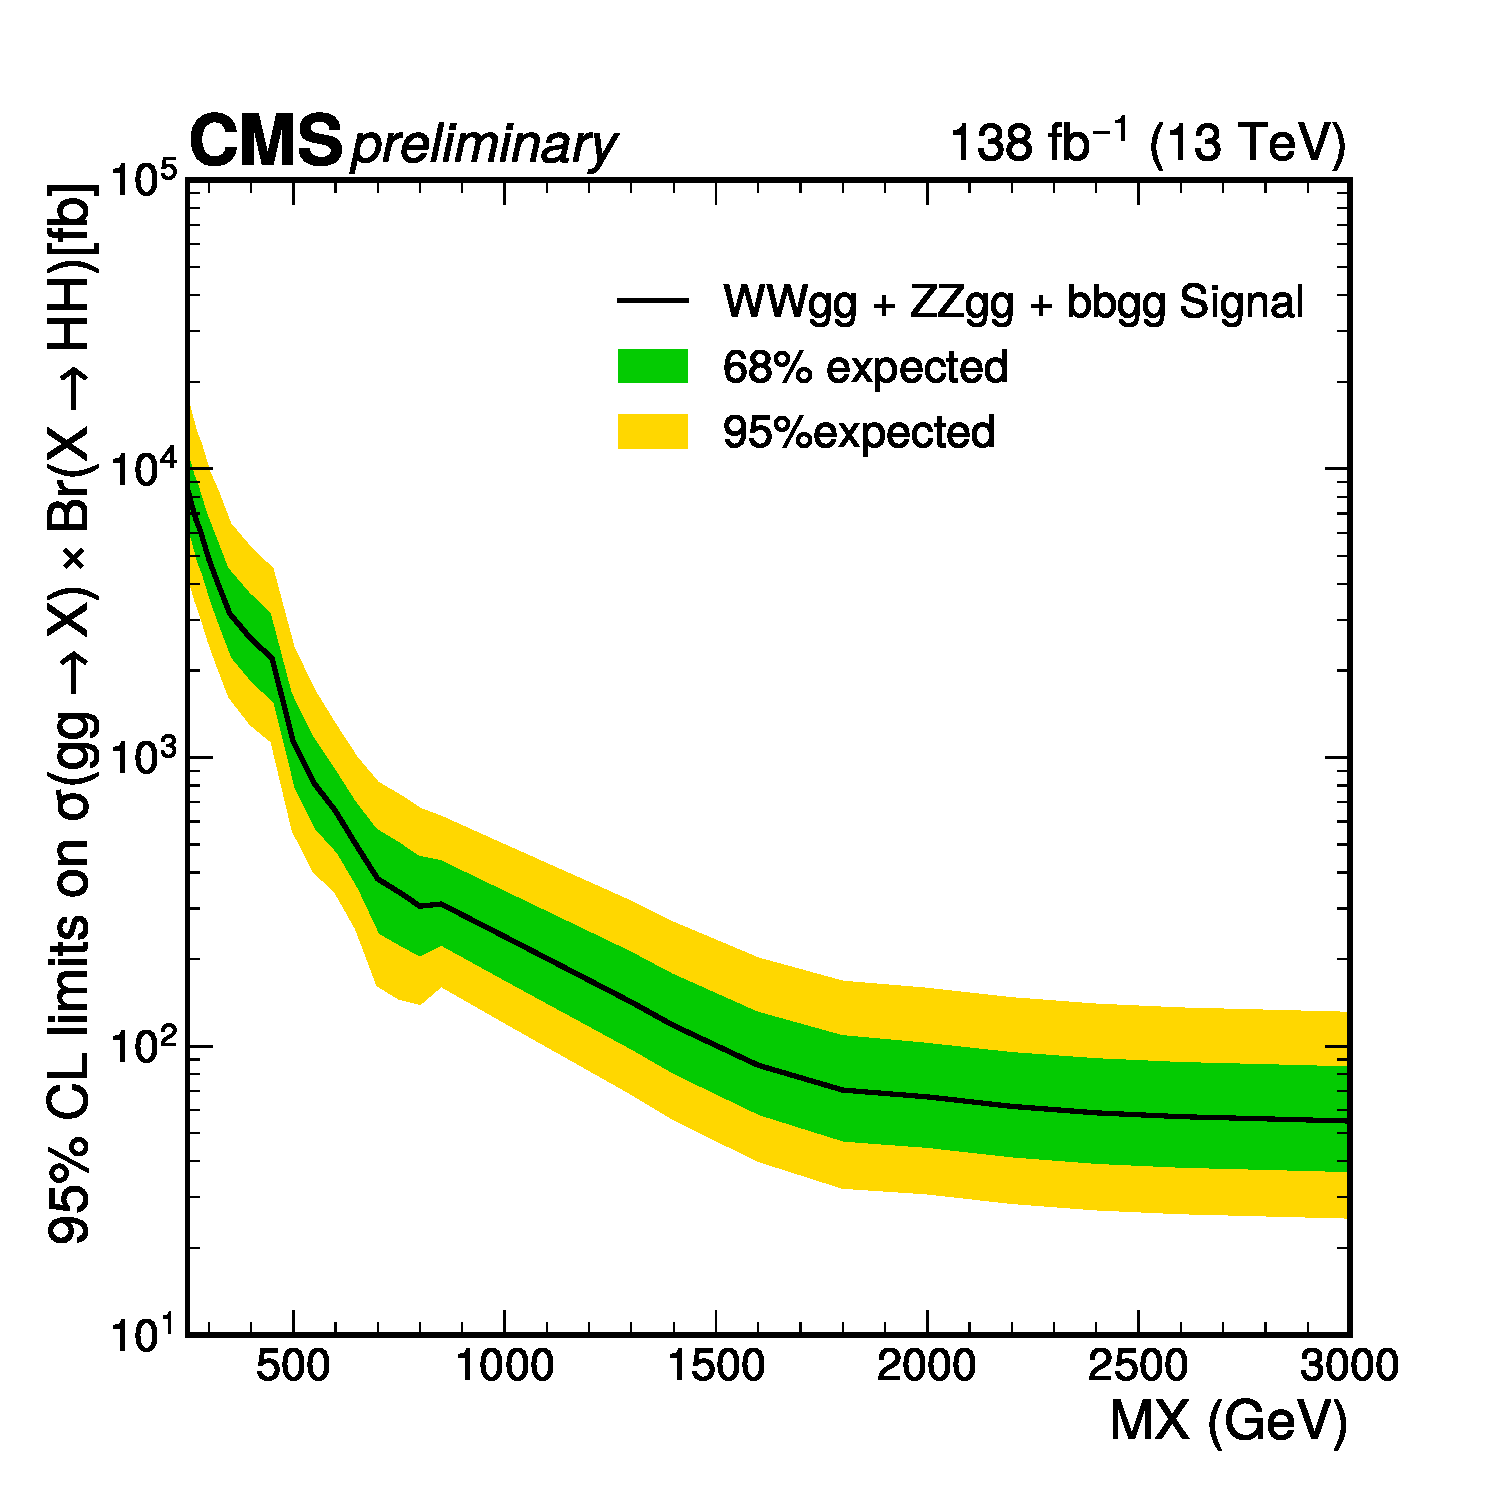
\includegraphics[width=0.8\textwidth]{figures/Limit/Run2_HH_limit.pdf}%
  \caption{Expected 95\% CL upper limits on the production cross-section times branching fraction ($\sigma \times \text{BR}$) for the resonant production of a spin-0 particle decaying into a Higgs boson pair.}
  \label{fig:limits_spin0}
\end{figure}

\begin{figure}[htbp!]
  \centering
  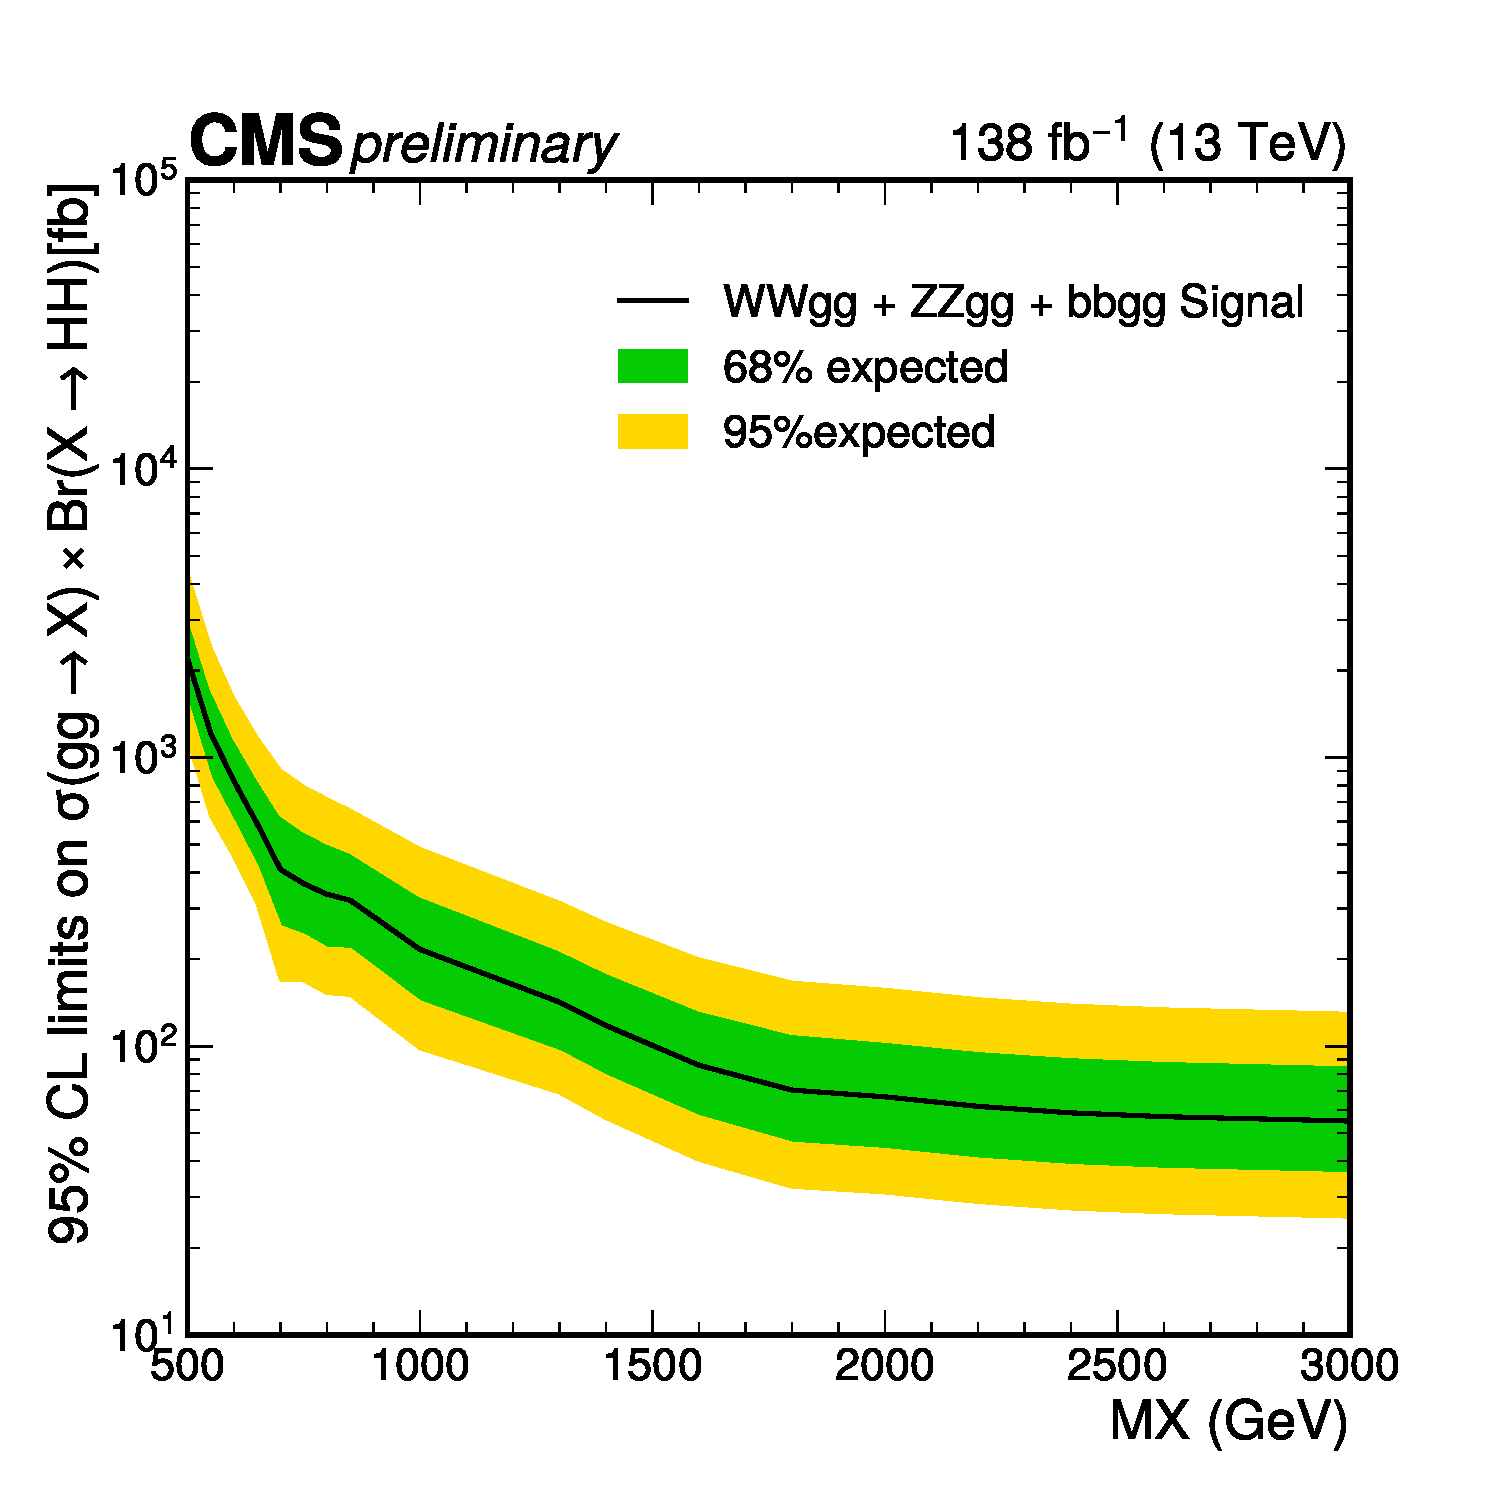
\includegraphics[width=0.4\textwidth]{figures/Limit/Run2_HH_limit_cat12.pdf}%
  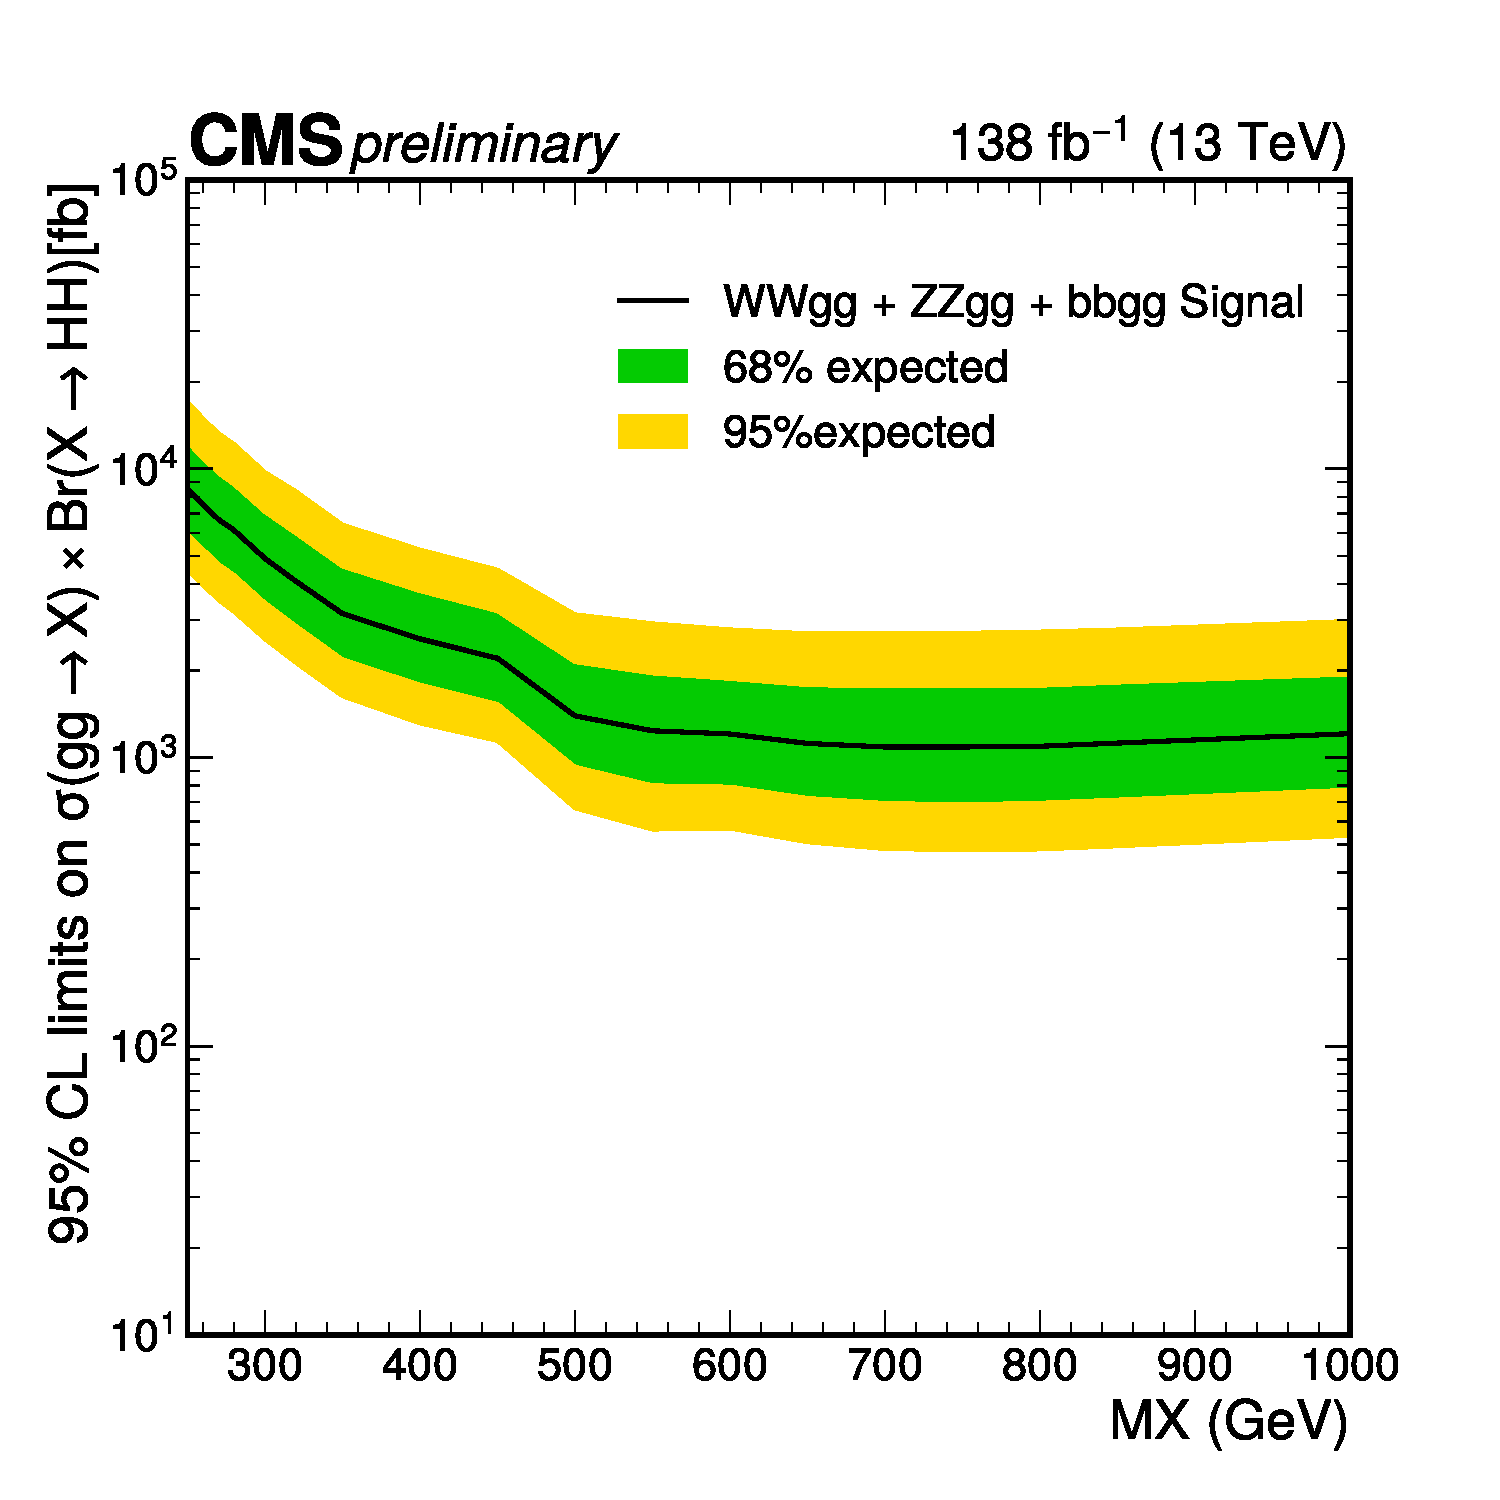
\includegraphics[width=0.4\textwidth]{figures/Limit/Run2_HH_limit_cat34.pdf}%

  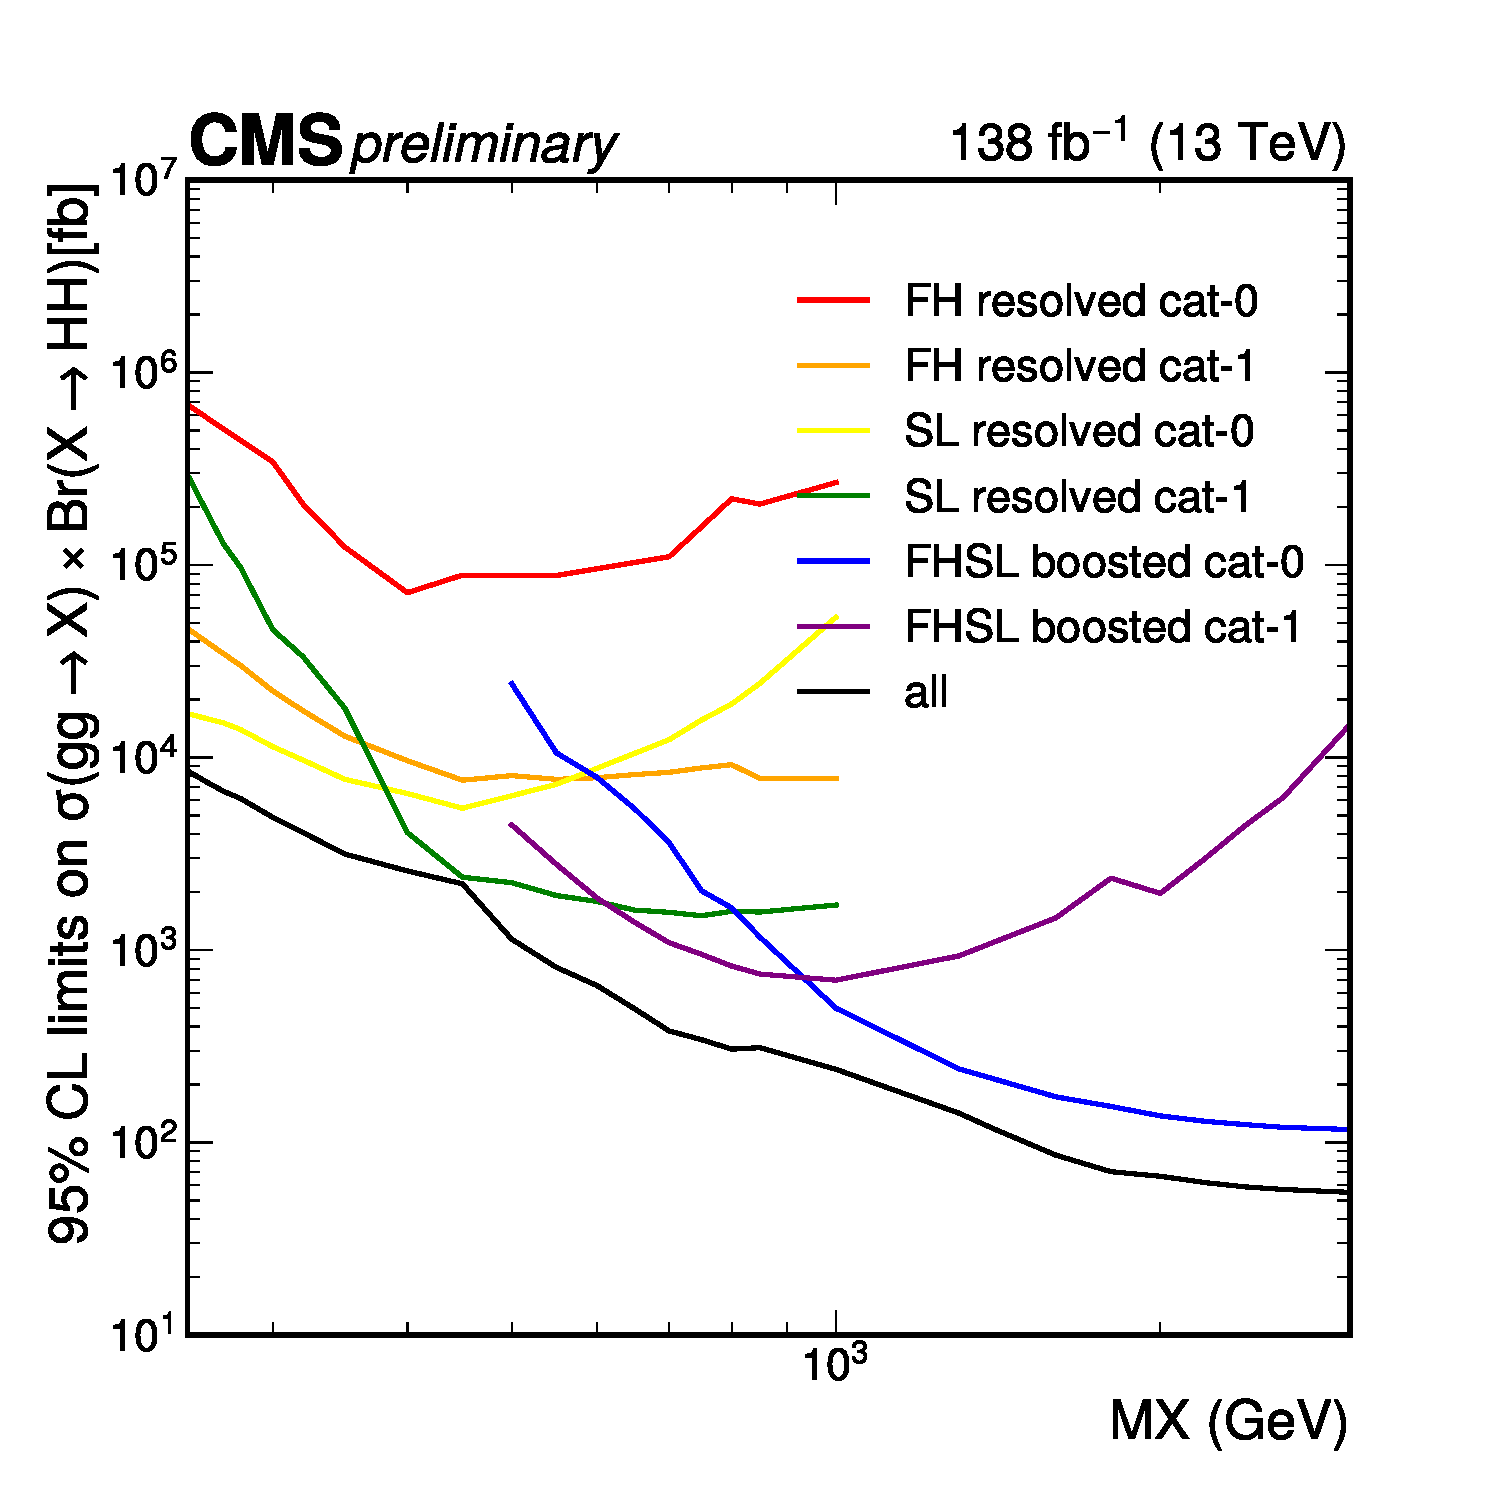
\includegraphics[width=0.75\textwidth]{figures/Limit/Run2_individual_cats_HH.pdf}%
  \caption{Individual expected 95\% CL upper limits on the production cross-section times branching fraction ($\sigma \times \text{BR}$) for the resonant production of a spin-0 particle decaying into a Higgs boson pair to the boosted(top left) and resolved(top right) categories and all sub-cateogries(bottom).}
  \label{fig:limits_separate}
\end{figure}



\section{Summary and Outlook}
This analysis represents the first CMS study of resonant di-Higgs production in the \(WW\gamma\gamma\) channel, incorporating all possible jet topologies and utilizing advanced machine learning techniques, such as parameterized neural networks. The findings place stringent constraints on Beyond Standard Model (BSM) scenarios that predict heavy resonances decaying into pairs of Higgs bosons.

Looking forward, the study aims to extend its scope to include non-resonant di-Higgs production with an additional scalar particle in the final state. These efforts will enhance sensitivity to di-Higgs processes and broaden the exploration of the Higgs sector, offering deeper insights into potential connections to new physics.
